%%%%%%%%%%%%%%%%%%%%%%%%%%%%%%%%%%%%%%%%%
% Short Sectioned Assignment
% LaTeX Template
% Version 1.0 (5/5/12)
%
% This template has been downloaded from:
% http://www.LaTeXTemplates.com
%
% Original author:
% Frits Wenneker (http://www.howtotex.com)
%
% License:
% CC BY-NC-SA 3.0 (http://creativecommons.org/licenses/by-nc-sa/3.0/)
%
%%%%%%%%%%%%%%%%%%%%%%%%%%%%%%%%%%%%%%%%%

%----------------------------------------------------------------------------------------
%	PACKAGES AND OTHER DOCUMENT CONFIGURATIONS
%----------------------------------------------------------------------------------------

\documentclass[paper=a4, fontsize=11pt]{scrartcl} % A4 paper and 11pt font size

\usepackage{listings}
\usepackage{color}

\definecolor{dkgreen}{rgb}{0,0.6,0}
\definecolor{gray}{rgb}{0.5,0.5,0.5}
\definecolor{mauve}{rgb}{0.58,0,0.82}

\lstset{frame=tb,
language=Java,
aboveskip=3mm,
belowskip=3mm,
showstringspaces=false,
columns=flexible,
basicstyle={\small\ttfamily},
numbers=none,
numberstyle=\tiny\color{gray},
keywordstyle=\color{blue},
commentstyle=\color{dkgreen},
stringstyle=\color{mauve},
breaklines=true,
breakatwhitespace=true,
tabsize=3
}

\usepackage[T1]{fontenc} % Use 8-bit encoding that has 256 glyphs
\usepackage[utf8]{inputenc}
\usepackage[spanish]{babel} % English language/hyphenation
\usepackage{amsmath,amsfonts,amsthm} % Math packages
% \usepackage{breakcites}
\usepackage{sectsty} % Allows customizing section commands
\allsectionsfont{\centering \normalfont\scshape} % Make all sections centered, the default font and small caps
\usepackage{algorithm}
\usepackage{url}
\usepackage[noend]{algpseudocode}
\makeatletter
\usepackage{graphicx}

\usepackage{fancyhdr} % Custom headers and footers
\pagestyle{fancyplain} % Makes all pages in the document conform to the custom headers and footers
\fancyhead{} % No page header - if you want one, create it in the same way as the footers below
\fancyfoot[L]{} % Empty left footer
\fancyfoot[C]{} % Empty center footer
\fancyfoot[R]{\thepage} % Page numbering for right footer
\renewcommand{\headrulewidth}{0pt} % Remove header underlines
\renewcommand{\footrulewidth}{0pt} % Remove footer underlines
\setlength{\headheight}{13.6pt} % Customize the height of the header
% Reinsert missing \algbackskip
\def\algbackskip{\hskip-\ALG@thistlm}
\renewcommand*{\ALG@name}{Algoritmo}
% \makeatother
\decimalpoint
\numberwithin{equation}{section} % Number equations within sections (i.e. 1.1, 1.2, 2.1, 2.2 instead of 1, 2, 3, 4)
\numberwithin{figure}{section} % Number figures within sections (i.e. 1.1, 1.2, 2.1, 2.2 instead of 1, 2, 3, 4)
\numberwithin{table}{section} % Number tables within sections (i.e. 1.1, 1.2, 2.1, 2.2 instead of 1, 2, 3, 4)

\setlength\parindent{0pt} % Removes all indentation from paragraphs - comment this line for an assignment with lots of text

%----------------------------------------------------------------------------------------
%	TITLE SECTION
%----------------------------------------------------------------------------------------

\newcommand{\horrule}[1]{\rule{\linewidth}{#1}} % Create horizontal rule command with 1 argument of height

\title{	
\normalfont \normalsize 
\textsc{Universidad Nacional de San Agustín, Escuela de Ingenieria de Sistemas} \\ [25pt] % Your university, school and/or department name(s)
\horrule{0.5pt} \\[0.4cm] % Thin top horizontal rule
\huge ADA - Lab 06 \\ % The assignment title
\horrule{2pt} \\[0.5cm] % Thick bottom horizontal rule
}

\author{Fernando Enrique Araoz Morales - 20173373} % Your name

\date{\normalsize\today} % Today's date or a custom date

\begin{document}

\maketitle % Print the title

%----------------------------------------------------------------------------------------
%	PROBLEM 1
%----------------------------------------------------------------------------------------

\section{Introducción}\label{sec:introducción}

En este documento se presenta la implementación de un algoritmo A*, usando como base la estructura
MinHeap construida con anterioridad.

El código de este y el resto de laboratorios se encuentra alojado en GitHub:

https://github.com/Araozu/ADA


    \section{Board}\label{sec:board}

    La clase Board representa el estado del tablero y cuenta con un atributo int[][] con las posiciones
    y un atributo Board que representa el tablero objetivo.

    El siguiente método de importancia es el método movesFrom(), el cual dado un elemento y una posición
    i y j (fila y columna) calcula la distancia entre la posición del elemento respecto a [i][j].

    El metodo manhattan() hace uso del método movesFrom() para obtener la distancia de Manhattan
    de todos los elementos del tablero.

    El método cloneBoard() clona el tablero actual para ser usado por el método swapAndReturn().
    Este método clona el tablero actual y en este intercambia un elemento por otro.

    Finalmente, el método neighbors() genera un ArrayList con todos los movimientos posibles respecto
    al elemento 0.

    \begin{lstlisting}


    import java.util.ArrayList;

    public class Board {

        private final int[][] board;
        private final Board goalBoard;

        // construct a board from an nxn array of blocks
        public Board(int[][] board, Board goalBoard) {
            if (board == null) {
                throw new IllegalArgumentException("The board is null.");
            }

            this.board = board;
            this.goalBoard = goalBoard;
        }

        public Board(int[][] board) {
            this(board, null);
        }

        public int[][] getBoard() {
            return board;
        }

        public boolean hasGoalBoard() { return goalBoard != null; }

        public Board getGoalBoard() {
            return goalBoard;
        }

        private int movesFrom(int elem, int i, int j) {
            int actualI = 0;
            int actualJ = 0;

            loop: for (; actualI < board.length; actualI++) {
                int[] row = board[actualI];
                for (; actualJ < row.length; actualJ++) {
                    if (row[actualJ] == elem) {
                        break loop;
                    }
                }
                actualJ = 0;
            }

            return Math.abs(i - actualI) + Math.abs(j - actualJ);
        }


        // sum of manhattan distances between blocks and goal
        public int manhattan() {
            if (goalBoard == null) return Integer.MAX_VALUE;

            int sum = 0;
            for (int i = 0; i < board.length; i++) {
                int[] row = board[i];
                for (int j = 0; j < row.length; j++) {
                    sum += goalBoard.movesFrom(row[j], i, j);
                }
            }

            return sum;
        }


        // is this board the goal board
        public boolean isGoal() {
            if (goalBoard == null) throw new NullPointerException("There is no goal board...");
            return this.equals(goalBoard);
        }

        // does this board equaly
        @Override
        public boolean equals(Object y) {
            if (!(y instanceof Board)) {
                throw new IllegalArgumentException("The object is not a Board.");
            }

            Board b = (Board) y;

            if (b.getBoard().length == board.length && b.getBoard()[0].length == board[0].length) {

                for (int i = 0; i < board.length; i++) {
                    for (int j = 0; j < board.length; j++) {
                        if (b.getBoard()[i][j] != board[i][j]) {
                            return false;
                        }
                    }
                }

                return true;
            } else {
                return false;
            }

        }

        private int[][] cloneBoard() {
            int[][] clone = new int[board.length][board[0].length];

            for (int i = 0; i < board.length; i++) {
                int[] row = board[i];
                System.arraycopy(row, 0, clone[i], 0, row.length);
            }

            return clone;
        }

        private int[][] swapAndReturn(int i1, int j1, int i2, int j2) {
            int[][] newBoard = cloneBoard();

            int buffer = newBoard[i1][j1];
            newBoard[i1][j1] = newBoard[i2][j2];
            newBoard[i2][j2] = buffer;

            return newBoard;
        }

        // all possible board generated from parent
        public ArrayList<Board> neighbors() {
            ArrayList<Board> res = new ArrayList<>();

            int zeroI = 0;
            int zeroJ = 0;

            loop: for (; zeroI < board.length; zeroI++) {
                int[] row = board[zeroI];
                for (; zeroJ < row.length; zeroJ++) {
                    if (row[zeroJ] == 0) {
                        break loop;
                    }
                }
                zeroJ = 0;
            }

            if (zeroI > 0) {
                int[][] copy = swapAndReturn(zeroI, zeroJ, zeroI - 1, zeroJ);
                res.add(new Board(copy, goalBoard));
            }

            if (zeroI < board.length - 1) {
                int[][] copy = swapAndReturn(zeroI, zeroJ, zeroI + 1, zeroJ);
                res.add(new Board(copy, goalBoard));
            }

            if (zeroJ > 0) {
                int[][] copy = swapAndReturn(zeroI, zeroJ, zeroI, zeroJ - 1);
                res.add(new Board(copy, goalBoard));
            }

            if (zeroJ < board[0].length - 1) {
                int[][] copy = swapAndReturn(zeroI, zeroJ, zeroI, zeroJ + 1);
                res.add(new Board(copy, goalBoard));
            }

            return res;
        }

        @Override
        public String toString() {
            String res = "";
            for (int[] row: board) {
                res += "[";
                for (int value: row) {
                    res += " " + value + " ";
                }
                res += "]\n";
            }

            return res;
        }

    }

    \end{lstlisting}

    \section{MinHeap}\label{sec:minheap}

    La clase MinHeap es un minHeap, pero a diferencia de la estructura presentada en el laboratorio
    anterior, esta usa un ArrayList debido a la necesidad de insertar y eliminar elementos
    constantemente.
    Los métodos principales son siftDown() que desplaza el elemento en la raiz del árbol a la
    posición que le corresponde, siftUp() desplaza un elemento insertado al final del ArrayList a la
    posición que le corresponde, y heapify() que dado un ArrayList inicial lo reordena para
    tener un minHeap.

    \begin{lstlisting}

    import java.util.ArrayList;

    public class MinHeap<T extends Comparable<T>> {

        private final ArrayList<T> arr;

        public MinHeap(ArrayList<T> arr) {
            this.arr = arr;
        }

        public MinHeap() {
        t   his(new ArrayList<>());
        }

        private void swap(int pos1, int pos2) {
            T buffer = arr.get(pos1);
            arr.set(pos1, arr.get(pos2));
            arr.set(pos2, buffer);
        }

        void heapify() {

            int lastPos = arr.size();
            int firstParent = (lastPos % 2 == 0)? (lastPos - 2) / 2: (lastPos - 1) / 2;

            for (int i = firstParent; i >= 0; i--) {
                siftDown(i, arr.size());
            }

        }

        private boolean compare(T a, T b) {
            return a.compareTo(b) < 0;
        }

        private void siftDown(int pos, int maxPos) {
            int largestPos = pos;
            int posLeft = pos * 2 + 1;
            int posRight = pos * 2 + 2;

            if (posLeft < maxPos && compare(arr.get(posLeft), arr.get(largestPos))) {
                largestPos = posLeft;
            }

            if (posRight < maxPos && compare(arr.get(posRight), arr.get(largestPos))) {
                largestPos = posRight;
            }


            if (largestPos != pos) {
                swap(pos, largestPos);

                siftDown(largestPos, maxPos);
            }

        }

        private void siftUp(int pos) {
            if (pos > 0) {

                int parentPos = (pos % 2 == 0)? (pos - 2) / 2: (pos - 1) / 2;
                if (compare(arr.get(parentPos), arr.get(pos))) {
                    swap(parentPos, pos);
                    siftUp(parentPos);
                }

            }
        }

        void sort() {
            this.heapify();
            for (int max = arr.size(); max > 0; --max) {
                swap(0, max - 1);
                this.siftDown(0, max - 1);
            }
        }

        public T removeHead() {
            T result = arr.get(0);
            arr.remove(0);

            if (arr.size() > 0) {
                swap(0, arr.size() - 1);
                this.siftDown(0, arr.size() - 1);
            }

            return result;
        }

        void insert(T elem) {
            arr.add(elem);
            heapify();
        }

        @Override
        public String toString() {
            StringBuilder res = new StringBuilder("[");
            for (T i: arr) {
                res.append(i).append(", ");
            }
            res.append("]");

            return res.toString();
        }


    }

    \end{lstlisting}

    \section{Solver}\label{sec:solver}

    Finalmente la clase Solver ejecuta el algoritmo A*. A sugerencia del profesor la lógica se
    encuentra íntegramente en el constructor, sin embargo, es necesario separar la funcionalidad
    en varios métodos.

    A la clase SearchNode se le ha incrementado una funcionalidad que permite recuperar el SearchNode
    padre.
    El resto se encuentra intacto.

    En el algorítmo en sí creamos un MinHeap<SearchNode> en el cual insertaremos los movimientos.
    Luego verificamos que el Board provisto:

    - No sea null.
    - Tenga un Board objetivo.
    - No sea igual al Board objetivo.

    A continuación procedemos a ejecutar un bucle mientras que el SearchNode con el que trabajamos
    no sea igual a la solución.

    Recuperamos el SearchNode con mayor prioridad del MinHeap, y de el obtenemos todos sus movimientos
    posibles, eliminando aquel movimiento que nos regrese a un estado anterior.

    Luego todos esos movimientos son agregados al MinHeap, y el proceso se repite.

    Cuando hemos encontrado el movimiento que coincide con la solución, procedemos a crear un Stack
    en el cual se van a insertar todos los pasos realizados hasta el momento, haciendo uso de la
    función crearSteps().

    Con ello concluye el algoritmo.
    El cliente es responsable de usar el Stack provisto para recuperar los pasos para llegar a
    la solución.

    \begin{lstlisting}

    import java.util.ArrayList;
    import java.util.Stack;

    public class Solver {
        private boolean solvable = false;
        private int moves;
        private Stack<Board> steps;

        private static class SearchNode implements Comparable<SearchNode> {
            private final Board board;
            private final int moves;
            private final SearchNode snode;
            private final int priority;

            public SearchNode(Board board, SearchNode predecessor) {
                this.board = board;

                if (predecessor != null) moves = predecessor.getMoves() + 1;
                else moves = 0;

                snode = predecessor;
                priority = moves + board.manhattan();
            }

            public int getMoves() {
                return moves;
            }

            public Board getBoard() {
                return board;
            }

            public SearchNode getpredecessor() {
                return snode;
            }

            public boolean hasParent() {
                return snode != null && snode.snode != null;
            }

            public Board getParent() {
                return snode.board;
            }

            public int getpriority() {
                return priority;
            }

            @Override
            public int compareTo(SearchNode sn) {
                if (priority > sn.getpriority()) {
                    return 1;
                }
                if (priority < sn.getpriority()) {
                    return -1;
                }
                if (priority == sn.getpriority()) {

                    if ((this.priority - this.moves) > (sn.priority - sn.moves)) {
                        return 1;
                    } else {
                        return -1;
                    }
                }
                return 0;
            }

        }

        public Solver(Board initial) {
            MinHeap<SearchNode> minpq = new MinHeap<>();

            if (initial == null)
                throw new IllegalArgumentException("Null argument");

            if (!initial.hasGoalBoard())
                throw new IllegalArgumentException("This board doesn't have a goal board.");


            if (initial.isGoal()) {

                solvable = true;
                steps = new Stack<>();
                steps.push(initial);

            } else {

                SearchNode actualNode = new SearchNode(initial, null);

                minpq.insert(actualNode);

                while (!actualNode.board.isGoal()) {

                    actualNode = minpq.removeHead();
                    ArrayList<Board> possibleMoves = actualNode.board.neighbors();

                    if (actualNode.hasParent()) {
                        Board grandFather = actualNode.getParent();

                        for (int i = 0; i < possibleMoves.size(); i++) {
                            if (possibleMoves.get(i).equals(grandFather)) {
                                possibleMoves.remove(i);
                                break;
                            }
                        }

                    }

                    for (Board b: possibleMoves) {
                        minpq.insert(new SearchNode(b, actualNode));
                    }

                }

                solvable = true;

                createSteps(actualNode);

            }

        }

        private void createSteps(SearchNode finalNode) {

            Stack<Board> stack = new Stack<>();

            SearchNode actualNode = finalNode;
            while (actualNode.snode != null) {
                stack.push(actualNode.board);
                actualNode = actualNode.snode;
            }
            stack.push(actualNode.board);

            this.steps = stack;

        }

        public boolean isSolvable() {
            return solvable;
        }

        public int moves() {
            return moves;
        }

        public Stack<Board> solution() {
        if (steps == null) return null;
            return steps;
        }

        public static void main(String[] args) {

            /*
            ArrayList<Integer> nums = new ArrayList<>();
            nums.add(1);
            nums.add(8);
            nums.add(5);
            nums.add(3);
            nums.add(2);
            nums.add(7);
            nums.add(6);
            nums.add(4);

            MinHeap<Integer> mh = new MinHeap<>(nums);
            System.out.println(mh);
            mh.heapify();
            System.out.println(mh);
            mh.insert(10);
            System.out.println(mh);
            mh.insert(-1);
            System.out.println(mh);
            */

            Board board1 = new Board(new int[][]{{0, 1, 2}, {3, 4, 5}, {6, 7, 8}});
            Board board2 = new Board(new int[][]{{0, 1, 6}, {7, 3, 2}, {4, 8, 5}}, board1);

            Solver s = new Solver(board2);

            Stack<Board> solution = s.solution();

            while(solution.size() > 0) {
                System.out.println(solution.pop());
            }

        }

    }

    \end{lstlisting}

% \begin{figure}
%     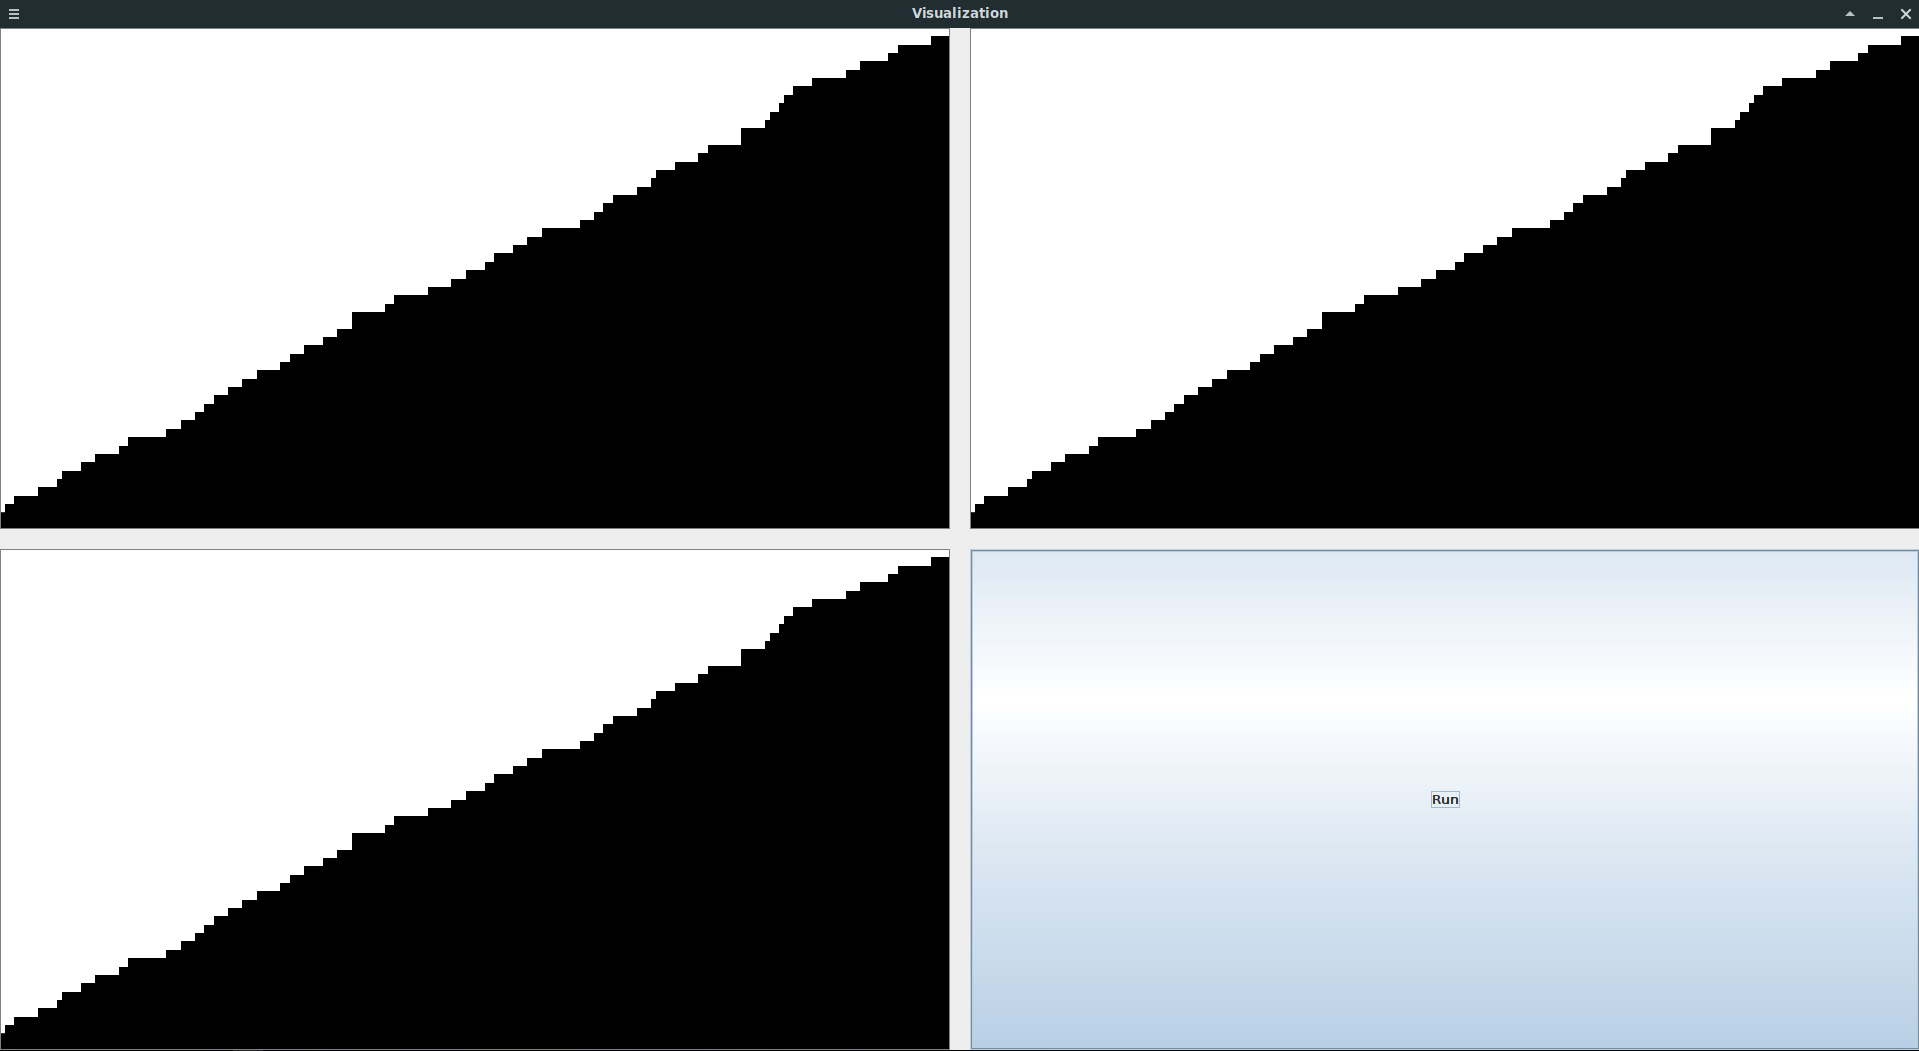
\includegraphics[width=\linewidth]{Resultado.png}
%     \caption{Resultado.}
% \end{figure}


%------------------------------------------------

\end{document}
